\section{A brief history of particle physics}

\graphicspath{{1_TheoreticalBackground/Figures}}

The understanding of the fundamental building blocks of the universe, which is known as particle
physics, has undergone a remarkable journey over the course of human history. The idea that all 
different forms of matter is composed of elementary particles is believed to date back to 
6th century BC. These elementary particles
were termed as ``atoms'', which originates from the Greek word ``atomos'' meaning ``indivisible''.
This view of matter is called \textit{atomism}, and it was argued that if it was possible to divide
matter into smaller blocks repeatedly, it would be then possible to reduce matter to nothing.
Hence, fundamental building blocks of matter, atoms, were necessary.
Experimental evidence for the atomic nature of matter started to emerge finally
in 19th century, when in 1815, English chemist William Prout noticed that the atomic masses
of many chemical elements were multiples of the mass of hydrogen, the lightest known element.
Hence, Prout hypothesized that all matter was built from hydrogen, suggesting hydrogen is the 
fundamental building block of matter. Although not being very accurate in today's understanding of atoms,
this was an important step (and the first significant experimental assertion) towards the understanding
of atoms as fundamental building blocks of matter.   

In the early 20th century however, it started to become apparent that
atoms are not indivisible solid entities themselves. J.J. Thomson discovered electrons (1897),
which were fundamental particles carrying negative electric charge~\cite{Thomson:1897cm}.
Shortly after, $\alpha$-particle scattering experiments by E. Rutherford et. al. (1909)~\cite{Rutherford:1911zz} 
revealed that at the center of each atom, a densely packed nucleus
must be located, carrying positive electric charge. From the results of the 
scattering experiments, Rutherford was able to deduce that the size of the nucleus $R_{n}$ must be $< 10^{-14}$ m.
Surrounding this dense nucleus, orbits of negatively charged electrons are located. It soon became clear that
the densely packed nucleus is not an indivisible object either, but is composed of positively charged 
protons~\cite{Rutherford:1919fnt}
and electrically neutral neutrons~\cite{Chadwick:1932ma}.

This model of atoms in which the negatively charged electrons are orbiting the nucleus 
has been challenged once again in 1920s when quantum mechanics (QM) was developed, which completely 
changed the understanding of how particles behave in atomic scales. The development of QM started 
at the turn of the 20th century. In an attempt to explain the photoelectric effect experiment by Hertz,
A. Einstein postulated that electromagnetic waves are composed of indivisible energy quanta, whose energy depends on the
frequency of the wave, $E = h\nu$ (1905)~\cite{Einstein:1905cc}. 
Here, $h$ refers to the Planck's constant (introduced in 1900 by M. Planck) and $\nu$
is the frequency of the electromagnetic wave. This understanding of the electromagnetic waves composed of identical 
particles (now called ``photons'') with small energy quanta led the way to the wave-particle duality, 
where each particle can be associated with a 
``matter wave''\footnote{The hypothesis that each particle has an associated wave with a wavelength inversely
proportional to their momentum, $\lambda = h / p$, is attributed to De Broglie (1924)~\cite{deBroglie:1924ldk}.}. 
E. Schrodinger (1926)~\cite{Schrodinger:1926gei} 
came up with a wave equation that describes the time evolution of this matter wave, denoted as $\Psi(\vec{x}, t)$, 
which is shown in Eq.~\ref{eq:schrodinger_eq}.

\begin{equation}
    i\hbar\frac{\partial \Psi(\vec{x}, t)}{\partial t} = \left(- \frac{\hbar^2}{2m}\nabla^2 + V(\vec{x}, t) \right)\Psi(\vec{x}, t)
    \label{eq:schrodinger_eq}
\end{equation}

where $\hbar = \frac{h}{2\pi}$ and $V(\vec{x}, t)$ describes the potential. 
It is worthy of note that Eq.~\ref{eq:schrodinger_eq} is a linear differential equation,
meaning a linear combination of solutions $\{ \Psi_{i} \}$ is itself also a solution.
The physical meaning of $\Psi(\vec{x}, t)$ however,
was not immediately obvious from Eq.~\ref{eq:schrodinger_eq}, it was eventually interpreted by 
M. Born (1926)~\cite{Born:1926uzf}
such that $|\Psi|^2$ is a probability density function that gives the probability to measure the particle
at a volume $V$ at time 
$t=t_{0}$:\footnote{It should be noted that this interpretation of $|\Psi|^2$ is not trivial and imposes important constraints
on possible forms of wave functions. $\Psi(x,t)$ must satisfy the condition 
$N(t) = \int_{-\infty}^{\infty} |\Psi(x,t)|^{2} dx = 1$ for all $t$.
It can be shown that if $\Psi$ satisfies $\lim_{x \rightarrow \pm \infty} \Psi(x,t) = 0$, and
$\lim_{x \rightarrow \pm \infty} \frac{\partial \Psi(x,t)}{\partial x} = K$ where $|K| < \infty$,
$\frac{dN(t)}{dt} = 0$ under the time evolution of $\Psi$ dictated by Eq.~\ref{eq:schrodinger_eq}. 
Hence, if $N(t_0) = 1$, $N(t) = 1$ for all $t > t_0$. The argument above
can be generalized to three space dimensions as well.}.

\begin{equation}
    P(t=t_0)  = \int_{V} d^3 x \ |\Psi(\vec{x}, t=t_0)|^2 
\end{equation}

Hence, with the advent of QM, determinism in the measurement of physical quantities of particles was lost.
One can only predict probabilities of mesaurements using the wave function $\Psi$, which can
be obtained from Eq.~\ref{eq:schrodinger_eq}. It should be noted that this is a very significant change 
of perspective (a ``paradigm shift'') compared to classical physics where each particle can be described
by a deterministic set of position and momenta coordinates $\{\vec{x}_i, \vec{p}_i\}$. 

It soon became apparent that there was a problem with Eq.~\ref{eq:schrodinger_eq}, namely that it was not compatible
with special relativity, which was proposed by A. Einstein (1905)~\cite{Einstein:1905ve} 
and described how the laws of physics are the same
in different frames of reference which move with constant velocities with respect to each other. The incompatibility
can be immediately observed by noticing the second-order space derivatives and the first-order time derivative in
Eq.~\ref{eq:schrodinger_eq}, which shows that the differential equation treats space and time coordinates differently.
P. Dirac (1928)~\cite{Dirac:1928hu} managed to write a differential equation with both first-order space and 
time derivatives, and is compatible
with the energy-momentum relationship from special relativity, $E^2 = p^2 c^2 + m^2 c^4$. This led to the Dirac equation,
shown in Eq.~\ref{eq:dirac_eq}.

\begin{equation}
    \left( i\hbar \gamma^{\mu} \partial_{\mu} - mc \right) \psi = 0
    \label{eq:dirac_eq}
\end{equation}

As with later equations in this thesis, Einstein summation convention is assumed in Eq.~\ref{eq:dirac_eq},
where it is implied that the repeated indices ($\mu$) are summed over.
The $\gamma$-matrices in Eq.~\ref{eq:dirac_eq} are a set of four $4\times 4$ matrices 
which satisfy the anti-commutation relation

\begin{equation}
    \{\gamma^{\mu}, \gamma^{\nu} \} = 2g^{\mu\nu}
\end{equation}

where $g^{\mu\nu}$ is the Minkowski metric tensor.
Dirac equation is a remarkable result and it has very important implications.
It predicts an internal property of particles called spin, 
which refers to the intrinsic angular momentum of a particle and has been
experimentally confirmed~\cite{Dirac:1928hu}. In addition, Eq.~\ref{eq:dirac_eq} has solutions with negative
energies, which was not immediately understood at the time\footnote{It is interesting to note
that the negative energy electron was initially thought to be corresponding to a proton,
for example see~\cite{Weyl:1929fm}. However, Dirac falsified this hypothesis
in 1930~\cite{Dirac:1930ek}.}. 
Ultimately, it was understood that those solutions described
antiparticles, which are counterparts of particles with the opposite electric 
charge~\footnote{The physical motivation behind this interpretation can be seen 
in this explanation by Dirac himself~\cite{Dirac:1930ek}: 
``... an electron with negative energy moves in an external
field as though it carries a positive charge.''}. 
In 1932, about four years later, positron (antiparticle of electron) 
was the first antiparticle to be discovered~\cite{Anderson:1932zz}. 
It is worthy of note that by combining principles of QM and special relativity,
Eq.~\ref{eq:dirac_eq} was able to predict these very fundamental physics.
Combination of QM with special relativity ultimately resulted in the development of 
Quantum Field Theory (QFT), which provides the mathematical framework 
of how we understand particles and their interactions to date.

By the beginning of 1960s, larger number of particles including
pions and kaons were discovered. Initially, these particles were all thought to 
be fundamental in nature~\cite{Riordan:1992hr}. 
However, as the number of known particles grew larger and larger, it came into 
question whether there could be
underyling elementary particles that make up all of these observed particles. This led 
Gell-Mann and Zweig to introduce quarks~\cite{Gell-Mann:1964ewy}, which are proposed to
be elementary particles making up the observed particles. Gell-Mann and Zweig proposed 
three types of quarks:
Up (u), down (s) and strange (s) quarks, together with their antiquark counterparts.
The particles made up by combining a quark and an antiquark are called mesons, while the particles made
from combining three quarks are termed baryons. Using this approach, Gell-Mann and Zweig were able to
explain all the known baryons and mesons, they even predicted new particles which would be discovered 
later\cite{Riordan:1992hr}. Going further in time, three more types of quarks (and corresponding 
antiquarks) were measured in addition to u, d and s: The charm quark c in 1974~\cite{E598:1974sol}, the
bottom (or beauty) quark b in 1977~\cite{E288:1977xhf} and finally the top quark t in 1995~\cite{D0:1995jca}.

The current understanding of these particles and their interactions are described by a group of quantum
field theories, which is called the Standard Model (SM). SM describes the electromagnetic, weak and 
strong nuclear interactions between these particles. A brief overview of the SM will be given in the
next section.

\section{The Standard Model of particle physics}

The Standard Model (SM) of particle physics describes different classes of known particles and their interactions
with each other, using QFT as the mathematical framework. It was developed in the second half of the 20th century
and has been very successful in predicting a wide variety of experimental observations. The development of the SM
was led by Chen Ning Yang, Robert Mills, Sheldon Glasgow, Steven Weinberg, and Abdus Salam.

In the SM, the strong interaction is derived by requiring Eq.~\ref{eq:dirac_eq} to be invariant under SU(3)
local phase transformations. The conserved quantum number of this symmetry is called color, and the quantum
field theory describing the color interaction of quarks and gluons is called Quantum Chronodynamics (QCD).
The SU(3) local phase transformations on a spinor $\psi$ can be written in the following form:

\begin{equation}
    \psi(x) \rightarrow \psi'(x) = \text{exp} \left[ i g_S \vec{\alpha}(x) \cdot \hat{\mathbf{T}}  \right]  \psi(x)
\end{equation}

where $\hat{\mathbf{T}} = \{ T^a \}$ are the eight generators of the SU(3) symmetry group and $\alpha^a(x)$ are eight functions
of the space-time coordinate $x$. $g_S$ is the coupling constant for the QCD interaction, which describes the strength
of the interaction. 
The invariance of Eq.~\ref{eq:dirac_eq} under local SU(3) transformations can be asserted by introducing eight new fields
$G_{\mu}^{a}(x)$, the index $a = 1, \dots, 8$ corresponding to one of the eight generators of the SU(3) symmetry, which
physically correspond to the eight possible gluon states in 
QCD\footnote{The gauge invariance is asserted given that the gluon fields $G_{\mu}^{k}$ transform as
$G_{\mu}^{k'} = G_{\mu}^{k} - \partial_{\mu}\alpha_{k} - g_{S}f_{ijk}\alpha_{i}G_{\mu}^{j}$, where $f_{ijk}$ are
the fine structure constants of the SU(3) group. The last term arises due to generators of SU(3) symmetry not commuting
with each other, and gives rise to gluon self-interactions.}.

The QCD interaction between quarks and gluon fields $G_{\mu}^{a}$ can be written in terms of the Lagrangian formalism.
The gluon field strength tensor, $G_{\mu\nu}^i$ can be defined as

\begin{equation}
    G_{\mu\nu}^i = \partial_{\mu}G_{\nu}^i - \partial_{\nu}G_{\mu}^i + g_{S} f^{ijk} G_{\mu}^{j} G_{\nu}^{k}
    \label{eq:gluon_field_strength}
\end{equation}

where $f^{ijk}$ refer to the fine structure constants of the SU(3) group, which can be defined by using the
commutators of the generators of SU(3) group $\{ T^{i} \}$ using the following relation: 
$[ T^{i}, T^{j} ] = i f^{ijk} T^{k}$. 
Using the gluon field strength tensor defined in Eq.~\ref{eq:gluon_field_strength}, 
the Lagrangian for the QCD interaction can be written as

% \begin{equation}
%     \mathcal{L}_{QCD} = \bar{\psi_{i}} \left( i \gamma^{\mu} (D_{\mu})_{ij} - m \delta_{ij} \right) \psi_{j} - \frac{1}{4} G_{\mu\nu}^{a} G^{\mu\nu}_{a}
% \end{equation}

\begin{equation}
    \mathcal{L}_{QCD} = \sum_{\psi} \left[ i \gamma^{\mu} \bar{\psi} \left( \partial_{\mu} - i g_{S} G_{\mu}^{a} T^{a} \right) \psi \right] - \frac{1}{4} G_{\mu\nu}^{a} G^{\mu\nu}_{a}
    % \mathcal{L}_{QCD} = \bar{\psi_{i}} \left( i \gamma^{\mu} (D_{\mu})_{ij} - m \delta_{ij} \right) \psi_{j} - \frac{1}{4} G_{\mu\nu}^{a} G^{\mu\nu}_{a}
\end{equation}

$\mathcal{L}_{QCD}$ characterizes the interaction between the gluon fields $G_{\mu}^{a}$ and quark spinors $\psi$.
The sum over $\psi$ indicates the sum over the spinors of quarks from different flavors.
Adjoint spinor $\bar{\psi}$ for each type of quark is defined as $\bar{\psi} = \psi^{\dag} \gamma^0$.
$\gamma^{\mu}$ are the set of four $4 \times 4$ matrices from Eq.~\ref{eq:dirac_eq}. 

The electroweak sector of the SM describes the electromagnetic and weak interactions between particles in a unified manner. The electroweak interaction
can be deduced by requiring the invariance of Eq.~\ref{eq:dirac_eq} under SU(2) x U(1) local phase transformations. 
This invariance can be asserted by introducing four
new fields, $W_{\mu}^{a}$ ($a = 1, 2, 3$) and $B_{\mu}$. The force carrier bosons of the weak interaction, $W^{+}, W^{-}, Z$ and the force carrier boson 
for the electromagnetic interaction, $\gamma$, can be then expressed in terms of these four fields. Fields for the $W^{\pm}$ bosons can be expressed as

\begin{equation}
    W^{\pm}_{\mu} = \frac{1}{\sqrt{2}} \left( W^{1}_{\mu} \pm i W^{2}_{\mu} \right)
\end{equation}

In addition, fields for $Z$ and $\gamma$ bosons can be written in terms of a mixing between $W_{\mu}^{3}$ and $B_{\mu}$ fields, 
as shown below in Eq.~\ref{eq:z_and_gamma_mixing}.

\begin{equation}
    \begin{pmatrix}
        \gamma_{\mu} \\ Z_{\mu}
    \end{pmatrix}
    = 
    \begin{pmatrix}
        \cos \theta_{W} & \sin \theta_{W} \\ 
        - \sin \theta_{W} & \cos \theta_{W}
    \end{pmatrix}
    \begin{pmatrix}
        B_{\mu} \\ W^{3}_{\mu}
    \end{pmatrix}
    \label{eq:z_and_gamma_mixing}
\end{equation}

where $\theta_{W}$ is the weak mixing angle. Experimental measurements provide $\sin^2 \theta_{W} = 0.23101 \pm 0.00053$~\cite{CMS:WeakMixingAngleMeasurement}.
Similar to gluon field strength tensor $G_{\mu\nu}^{i}$, one can write the field strength tensors for these four fields as $W_{\mu\nu}^{i}$ and $B_{\mu\nu}$ as

\begin{equation}
    \begin{split}
        W_{\mu\nu}^{i} &= \partial_{\mu} W_{\nu}^{i} - \partial_{\nu} W_{\mu}^{i} - g_{W} \epsilon^{ijk} W_{\mu}^{j} W_{\nu}^{k} \\
        B_{\mu\nu}     &= \partial_{\mu} B_{\nu}     - \partial_{\nu} B_{\mu}
    \end{split}
    \label{eq:field_strength_ew}
\end{equation}

The extra term in $W_{\mu\nu}^{i}$ should be noted to be arising from the non-commuting nature of SU(2) generators.
The Lagrangian describing the interactions of $W_{\mu}^{a}$ and $B_{\mu}$ fields can then be written as

\begin{equation}
    \mathcal{L}_{g} = -\frac{1}{4} W_{\mu\nu}^{a} W^{\mu\nu}_{a} -\frac{1}{4} B_{\mu\nu} B^{\mu\nu}
    \label{eq:lagrangian_kinetic_term}
\end{equation}

The full electroweak Lagrangian describing the electroweak interactions of $W_{\mu}^{a}$ and $B_{\mu}$ fields
with fermion fields can be in turn written as

\begin{equation}
        \mathcal{L}_{f}  = \sum_{\psi} \bar{\psi} \gamma^{\mu} \left( i \partial_{\mu} - g' \frac{1}{2} Y_{W} B_{\mu} - g \frac{1}{2} \sigma_{a} W_{\mu}^{a} \right) \psi
    \label{eq:ew_lagrangian_fermion_interactions}
\end{equation}

In Eq.~\ref{eq:ew_lagrangian_fermion_interactions}, $\psi$ refers to the SU(2) doublets of chirally left-handed particles and SU(2) singlets
of right-handed particles, highlighting the unequal coupling of $W_{\mu}^{i}$ and $B_{\mu}$ fields to left-handed and right-handed fermions.
This is also a crucial fact that is experimentally verified by C. S. Wu in 1956~\cite{Wu:1957my}. Finally, the full electroweak Lagrangian
$\mathcal{L}_{EW}$ can be written as the sum of Eqs.~\ref{eq:lagrangian_kinetic_term} and~\ref{eq:ew_lagrangian_fermion_interactions}:

\begin{equation}
    \mathcal{L}_{EW} = \sum_{\psi} \bar{\psi} \gamma^{\mu} \left( i \partial_{\mu} - g' \frac{1}{2} Y_{W} B_{\mu} - g \frac{1}{2} \sigma_{a} W_{\mu}^{a} \right) \psi - \frac{1}{4} W_{\mu\nu}^{a} W^{\mu\nu}_{a} -\frac{1}{4} B_{\mu\nu} B^{\mu\nu}
    \label{eq:ew_lagrangian}
\end{equation}

It should be noted that in Eq.~\ref{eq:ew_lagrangian}, there are no mass terms for the $W$ and $Z$ bosons (in the form $W_{\mu} W^{\mu}$)
which are known to be massive. However, inclusion of such terms in the Lagrangian would break the SU(2) x U(1) symmetry, hence the fermions
and gauge bosons have to acquire mass through a different mechanism. In the SM, this mechanism is called the Higgs mechanism, which introduces
a new scalar field called Higgs field, which can be written as a doublet as shown below:

\begin{equation}
    \phi = \frac{1}{\sqrt{2}} \begin{pmatrix}
        \phi^{+} \\ \phi^{0}
    \end{pmatrix}
    \label{eq:higgs_doublet}
\end{equation}

With the Higgs doublet $\phi$ defined in Eq.~\ref{eq:higgs_doublet}, the Higgs-sector Lagrangian can be written as

\begin{equation}
    \mathcal{L}_{Higgs} = \left[ \left( \partial_{\mu} - i \frac{g}{2} W_{\mu}^{a} \sigma_{a} - ig' Y_{\phi} B_{\mu} \right) \phi \right]^{2} + \mu^2 \phi^{\dag} \phi - \lambda \left( \phi^{\dag} \phi \right)^{2}
    \label{eq:higgs_lagrangian}
\end{equation}

In the unitarity gauge, one can set $\phi^{+} = 0$ and make $\phi^{0}$ real in the doublet of Eq.~\ref{eq:higgs_doublet}, hence writing $\phi$ as
$\phi(x) = \frac{1}{\sqrt{2}} \begin{pmatrix} 0, & v + h(x) \end{pmatrix}$. 
Then, $\langle \phi^{0} \rangle = v$ is the non-zero vacuum expectation value of the Higgs field, and the fluctuations around $\psi_{0} = v$
(i.e. $h(x)$) describes a new boson (i.e. the Higgs boson). Writing Eq.~\ref{eq:higgs_lagrangian} with $\phi$ in the unitary gauge, 
quadratic terms in $W_{\mu}$ and $B_{\mu}$ arise, giving mass to $W$ and $Z$ bosons:

\begin{equation}
    M_{W} = \frac{1}{2} v g, \qquad M_{Z} = \frac{1}{2} v \sqrt{g^2 + g'^{2}}
\end{equation}

The mass of the Higgs boson itself is then given by $M_{H} = \sqrt{2 \mu^2} = \sqrt{2 \lambda v^2}$. Through Yukawa couplings between fermions and the
Higgs field, it can be shown that fermions also acquire mass due to the non-zero expectation value $v$ 
of the Higgs field\footnote{Writing the Higgs doublet as $\phi(x) = \frac{1}{\sqrt{2}} \begin{pmatrix} 0 \\ v + h(x) \end{pmatrix}$, it can be shown that
Lagrangian acquires terms $\mathcal{L}_{f} = -m_{f} \bar{f} f - \frac{m_f}{v} \bar{f} f h $. Here, the first term is the mass term, which
represents the coupling of the fermion $f$ to the Higgs field through the non-zero expectation value of the Higgs field.
The second term represents the coupling of $f$ to the Higgs boson itself.}. In this way, the observed masses of the weak bosons ($W^{\pm}, Z$)
and fermions can be explained successfully with the SM.

In summary, the Standard Model (SM) can explain the strong and electroweak interactions between particles through the use of QFT as the mathematical framework.
All the known particles in the SM and their interactions are summarized in Fig.~\ref{fig:sm_interactions}. SM has been proven to be a very successful theory,
predicting a variety of physics phenomena that has been observed in particle physics experiments over the last decades.
The detection of $W^{\pm}$ and $Z$ bosons~\cite{UA1:WBosonDiscovery} was a crucial test of the electroweak sector of the SM. In fact,
the mass of these bosons as predicted by the SM, $M_W = 80357 \pm 6$ MeV and $M_Z = 91188 \pm 2$ MeV, 
are in very good agreement with the experimentally measured values~\cite{ATLAS:WMassMeasurement, CMS:ZMassMeasurement}. In addition,
the Higgs boson (H) (predicted by the Higgs mechanism) was observed in 2012 by ATLAS and CMS experiments~\cite{Nisati:2015iwc}, and the 
measured properties of the Higgs boson have so far been consistent with the SM predictions~\cite{CMS:2022dwd}. 

\begin{figure}[htbp]
    \centering
    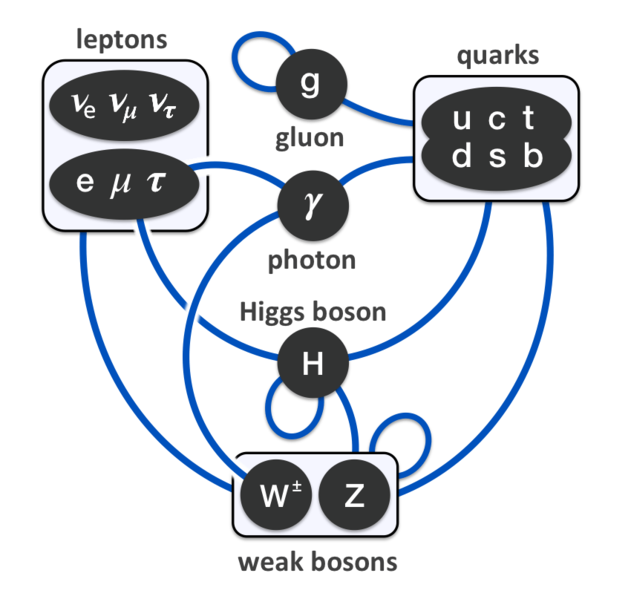
\includegraphics[width=0.9\textwidth]{SM_interactions.png}
    \caption{Schematic illustrating all the known particles in the SM and their interactions. Connections between different
    particles indicate that they interact. For the weak bosons ($W^{\pm}, Z$), gluons and the Higgs boson, self-interactions
    are also shown. Diagram is drawn by Eric Drexler.}
    \label{fig:sm_interactions}
\end{figure}

\clearpage